%%%%%%%%%%%%%%%%%%%%%%%%%%%%%%%%%%%%%%%%%%%%%%%%%%%%%%%%%%%%%%%%%%%%%%%%
%                                                                      %
%     File: Thesis_Implementation.tex                                  %
%     Tex Master: Thesis.tex                                           %
%                                                                      %
%     Author: Andre C. Marta                                           %
%     Last modified : 13 May 2019                                      %
%                                                                      %
%%%%%%%%%%%%%%%%%%%%%%%%%%%%%%%%%%%%%%%%%%%%%%%%%%%%%%%%%%%%%%%%%%%%%%%%

%	Daqui para a frente, apresenta-se a implementação de cada um dos módulos, com os respectivos resultados.

\chapter{Global path planner}
\label{chapter:implementation}

In order to feed the control system with a reference path, an offline survey of the target environment is conducted in order to generate a \tb{traversability cost map}, which performs an analysis of the terrain uneveness with respect to the robot kinematics and geometric features. Then, the same \tb{cost map} is fed to the Eikonal equation in order to yield a gradient potential map, where an optimal path to some goal position is retrieved.

%%%%%%%%%%%%%%%%%%%%%%%%%%%%%%%%%%%%%%%%%%%%%%%%%%%%%%%%%%%%%%%%%%%%%%%%
\section{Traversability map computation}
\label{section:costMap}

As mentioned in subsection \ref{subsection:worldModelling}, there is no explicit guideline on how to generate a traversability map. In this thesis, several approaches are compared. First, the state-of-the art algorithm from \cite{Amorim2014} is reviewed and evaluated. Then, this algorithm is reformulated to account for other metrics such as terrain inclination and roughness \cite{Ishigami2007PathPlanning}.

\subsection{Height minimization}
\label{subsection:heightMinimization}

A constrained optimization problem which minimizes the height of the robot at each cell is described. It is very similar to the solution provided in \cite{Amorim2014}. In this case, a wheeled vehicle is used instead of a tracked one. The yaw angle is set as a fixed variable and the initial guess $\boldsymbol{\upsilon}_0$ of the problem at every cell is set by an approximation to the optimal solution.

\subsubsection*{Initial guess}

Provided that the yaw angle $\yaw$ and the $\x$ and $\y$ position coordinates are known, each wheel point is projected to $\Map_2$. Then, from the group of retrieved contact points, the lowest height one is discarded, and an unit, normal vector to a plane which contains these points, is computed. Finally, the roll and pitch of this plane are given by equation \ref{eq:rollPitchInitialGuess}, where $\left( a, \, b, \, c \right)$ are the coordinates of a normal vector to the above mentioned plane. In case any of these angles are higher than $\roll_{max}$ or $\pitch_{max}$, the respective angle is set to the highest admissable value, so that the initial guess is feasible. The height initial guess $\z_0$ is set as the sum of the projection of the robot center of mass point to $\Map_2$ plus the robot geometric height, to avoid any possible intrusion of the vehicle hull into the ground.

\begin{equation}
	\begin{aligned}
		\roll &= \arcsin \left( \sin(\yaw) \, a -\cos(\yaw)\, b \right) \\
		\pitch &= \arccos \left( \frac{c}{\cos\left( \roll \right)} \right) \\
	\end{aligned}	
	\label{eq:rollPitchInitialGuess}
\end{equation}

\subsubsection*{\acrlong{nlp}}

The minimization of the vehicle \acrlong{com} is expressed as a non-linear optimization problem (\acrshort{nlp}) in equation \ref{eq:minHeight}, where $\boldsymbol{\Orientation}_{max}$ stands as the limits for each euler angle. $\mathbf{p}_k$ stands as the $k$ hull point position, which is defined with respect to $\WorldFrame$, by taking into account the robot geometry. $[\x, \y, \yaw]^T$ are fixed variables whereas $\left[ {\z},\, {\roll},\, {\pitch}\right]^T$ are set as optimization variables. Each point included in \ref{eq:minHeight} adds an additional constraint by stating each hull point must be above or at contact with the terrain. In case less than three hull points (each one from a different wheel) are at contact with the terrain, the terrain inclination returned by algoritm \ref{alg:slopeMinHeight} is $\frac{\pi}{2}$. This expresses the fact that the robot will stand at an unstable position, so this position is regarded as an undesirable traversable position.  On the other hand, the terrain inclination is given by equation \ref{eq:inclination}, which returns the angle between a normalized vector with direction $\BodyFrame_z$ and the normalized vector $\WorldFrame_z$ \cite{Amorim2014}. Although algorithm \ref{alg:slopeMinHeight} can be extended to any kind of wheeled-mobile robot configuration, only four wheel mobile robots are considered in this thesis, as mentioned in section \ref{section:problemFormulation}.

\raisebox{2ex}
{
	\begin{minipage}[c]{0.35\linewidth}
    \centering
    \begin{eqnarray}
  		{\rm Minimize}   && J = \z \nonumber \\
  		{\rm w.r.t.}     && \boldsymbol{\upsilon} = \left( {\z},\, {\roll},\, {\pitch} \right) \nonumber \\
  		{\rm subject~to} && \forall_k: \z_k - \FunctionElevation(\x_k, \y_k) \geq 0 \hspace{10mm} \label{eq:minHeight} \\
                   	 	 && \boldsymbol{\Orientation}_{max} - \left| \boldsymbol{\Orientation} \right| \geq 0 \, \nonumber
	\end{eqnarray}
	\begin{equation}
		\TraversabilityCost = \arccos( \cos(\pitch) \cos(\roll) )
		\label{eq:inclination}
	\end{equation}
  	\end{minipage}
}
\hfill
\raisebox{2ex}
{
	\begin{minipage}[c]{0.5\linewidth}
    \begin{algorithm}[H]
	\caption{\footnotesize Terrain inclination with \textsc{heightmin}}\label{alg:slopeMinHeight}
	\centering
	\footnotesize
	\begin{algorithmic}[1]
	\Function{terrainslope}{$\boldsymbol{\Orientation}_{max},\, \FunctionElevation(\cdot),\, \boldsymbol{\upsilon}_0,\, x,\, y, \, \yaw$}
	\State $\boldsymbol{\upsilon}_* \gets \textsc{heightmin}(\boldsymbol{\upsilon}_0, \, \boldsymbol{\Orientation}_{max},\, \FunctionElevation(\cdot), \,x, \,y, \, \yaw)$ \Comment{solve \ref{eq:minHeight}}
	\If{$\textmd{Contacts} \geq 3$}
	\State $\TraversabilityCost \gets \textsc{inclination}(\roll_*,\, \pitch_*)$ \Comment{\ref{eq:inclination}}
	\Else
	\State $\TraversabilityCost \gets \frac{\pi}{2}$
	\EndIf
	\State \Return $\TraversabilityCost, \, \boldsymbol{\upsilon}_*$
	\EndFunction
	\end{algorithmic}
	\end{algorithm}
	\end{minipage}
}

\begin{algorithm}[H]
	\caption{\footnotesize Terrain inclination map with \textsc{terrainslope}}\label{alg:slopeMinHeightMap}
	\centering
	\footnotesize
	\begin{algorithmic}[1]
	\Function{inclinationfixyaw}{$\boldsymbol{\Orientation}_{max}, \, \yaw, \, \FunctionElevation(\cdot), \,N_0,\, N_1$}
	\ForEach{$\{i,\,j\} \in \{0,\, \ldots, \, N_0 - 1\} \times \{0,\, \ldots, \, N_1 - 1\}$}
	\State $\boldsymbol{\upsilon}_0 \gets \textsc{initialguess}(x_i,\, y_j, \, \yaw)$ \Comment{feasible initialization}
	\If{$\RobotCircleHullArea_2 \subset \Map_2$}
	\State $\TraversabilityCost,\,\boldsymbol{\upsilon}_* \gets \textsc{terrainslope}(\boldsymbol{\Orientation}_{max},\, \FunctionElevation(\cdot),\,\boldsymbol{\upsilon}_0, x_i,\, y_j, \, \yaw)$ \Comment{algorithm \ref{alg:slopeMinHeight}}
	\Else
	\State $c \gets \frac{\pi}{2}$
	\EndIf
	\State $\FunctionTraversability_d(i,\, j) \gets c$
	\EndFor
	\State \Return $\FunctionTraversability_d(\cdot)$ 
	\EndFunction
	\end{algorithmic}
\end{algorithm}

Then, algorithm \ref{alg:slopeMinHeightMap} extends the application of algorithm \ref{alg:slopeMinHeight} to each cell of the elevation grid. It should be noted that the discrete elevation grid $\FunctionElevation_d(\cdot)$ shall have such dimensions that the cell divison length is smaller than the magnitude order of the wheel diameter in meters. Moreover, a convex area $\RobotCircleHullArea_2$ (equation \ref{eq:robotHullArea}) centered at $[x,\,y]^T$ which captures the robot hull $\RobotHullArea_2$ projection in $\Map_2$ must lie inside the map domain. If this condition is not met, the terrain inclination angle assigned to $\FunctionTraversability_d(\cdot)$ is $\frac{\pi}{2}$. Therefore, positions at which the assigned terrain inclination is $\frac{\pi}{2}$ are considered to be untraversable. To sum up, the higher the inclination, the less desirable it is to pass through the respective position.

\begin{equation}
	\RobotCircleHullArea_2 = \{ \text{min} \, \underline{h}: \| \mathbf{\Position}_2 - \mathbf{a} \| \leq \underline{h} \, | \, \mathbf{\Position}_2,\, \mathbf{a} \in \Map_2 , \, \mathbf{p}_{2, k} \in \RobotCircleHullArea_2 \}
	\label{eq:robotHullArea}
\end{equation}

\subsubsection*{Variable yaw}

The terrain traversability may also be assessed by finding the maximum inclination at each position by saving the maximum retrieved inclination among several yaws. Algorithm \ref{alg:slopeMinHeightMap} lacks a thorough evaluation of the terrain irregularity, as it changes depending on the mobile robot heading. In order to tackle this absence of completeness, algorithm \ref{alg:slopeMinHeightMap} is reformulated to address this issue. 

\begin{algorithm}[H]
	\caption{\footnotesize Terrain inclination map with \textsc{terrainslope} and variable yaw}\label{alg:slopeMinHeightMapVarYaw}
	\centering
	\footnotesize
	\begin{algorithmic}[1]
	\Function{inclinationvaryaw}{$\boldsymbol{\Orientation}_{max}, \, \FunctionElevation(\cdot), \,N_0,\, N_1$}
	\ForEach{$\{i,\,j\} \in \{0,\, \ldots, \, N_0 - 1\} \times \{0,\, \ldots, \, N_1 - 1\}$}
	\ForEach{$\yaw_k$} \Comment{variable yaw}
	\State $\boldsymbol{\upsilon}_0 \gets \textsc{initialguess}(x_i, \, y_j, \, \yaw_k)$ \Comment{feasible initialization}
	\If{$\RobotCircleHullArea_2 \subset \Map_2$}
	\State $\TraversabilityCost_k,\, \left( \boldsymbol{\upsilon}_* \right)_k \gets \textsc{terrainslope}(\boldsymbol{\Orientation}_{max}, \, \FunctionElevation(\cdot), \, \boldsymbol{\upsilon}_0, \, x_i, \, y_j, \, \yaw_k)$ \Comment{algorithm \ref{alg:slopeMinHeight}}
	\Else
	\State $\TraversabilityCost_k \gets \frac{\pi}{2}$
	\EndIf
	\EndFor
	\State $\TraversabilityCost \gets \text{max}\left( \TraversabilityCost_k \right)$ \Comment{save maximum inclination}
	\State $\FunctionTraversability_d(i,\, j) \gets \TraversabilityCost$
	\EndFor
	\State \Return $\FunctionTraversability_d(\cdot)$
	\EndFunction
	\end{algorithmic}
\end{algorithm}

In algorithm \ref{alg:slopeMinHeightMapVarYaw}, $\yaw_k = \lbrace -\pi,\, \ldots,\, -\pi + k \alpha, \, \ldots, \, \pi - \alpha \rbrace$, where $\alpha$ stands as the step angle of the set $\yaw_k$.

\subsection{Maximum terrain roughness}
\label{subsection:maxTerrainRoughness}

Terrain traversability may also be evaluated by inspecting terrain roughness around each position of the map, where the goal is to evaluate the maximum terrain uneveness at each position of the map. In this thesis, terrain roughness at each position of $\Map_2$ is defined as the standard deviation of elevations inside $\RobotHullArea_2$.

\begin{equation}
	\bar{\FunctionElevation}_d(i, j) = \frac{\sum_{\x_i,\,\y_j \in \RobotHullArea_2} \FunctionElevation(x_i, \, y_j)}{n(\underline{\RobotHullArea}_2)},\, \underline{\RobotHullArea}_2 = \{ \left( \x_i,\, \y_j \right) \in \RobotHullArea_2 \}  
	\label{eq:averageHeight}
\end{equation}

, where $\underline{\RobotHullArea}_2$ denotes a finite set of points from $\FunctionElevation_d(\cdot)$ inside $\RobotHullArea_2$ and $\bar{\FunctionElevation}_d(i, j)$ the average of elevations for points inside $\RobotHullArea_2$. Then, terrain roughness is defined as,

\begin{equation}
	\FunctionTraversability_d(i,\,j) = \sqrt{\frac{\sum_{\x_i,\,\y_j \in \RobotHullArea_2}{} \left( \FunctionElevation(i,\,j) - \bar{\FunctionElevation}(i,\,j) \right)^2 }{n(\underline{\RobotHullArea}_2)}}
	\label{eq:terrainRoughness}
\end{equation}

The set of points inside $\underline{\RobotHullArea}_2$ depends on the yaw angle of the mobile robot, so $\FunctionTraversability_d(i,\,j)$ is computed for each yaw angle. Similarly to what was done in algorithm \ref{alg:slopeMinHeightMapVarYaw}, the terrain roughness assigned to the respective cell is the maximum roughness among the set of yaws $\yaw_k$. Finally, a maximum terrain roughness may be computed by coding algorithm \ref{alg:maxRoughnessMap}.

\begin{algorithm}[H]
	\caption{\footnotesize Maximum terrain roughness map}\label{alg:maxRoughnessMap}
	\centering
	\footnotesize
	\begin{algorithmic}[1]
	\Function{roughness}{$\boldsymbol{\Orientation}_{max}, \, \FunctionElevation(\cdot), \,N_0,\, N_1$}
	\ForEach{$\{i,\,j\} \in \{0,\, \ldots, \, N_0 - 1\} \times \{0,\, \ldots, \, N_1 - 1\}$}
	\If{$\RobotCircleHullArea_2 \subset \Map_2$}
	\ForEach{$\yaw_k$} \Comment{variable yaw}
	\State $\TraversabilityCost_k \gets \text{equation} \left( \ref{eq:terrainRoughness} \right)$ \Comment{equation (\ref{eq:terrainRoughness})}
	\EndFor
	\Else
	\State $\TraversabilityCost_k \gets \texttt{None}$
	\EndIf
	\State $\TraversabilityCost \gets \text{max}\left( \TraversabilityCost_k \right)$ \Comment{save maximum roughness}
	\State $\FunctionTraversability_d(i,\, j) \gets \TraversabilityCost$
	\EndFor
	\State \text{Replace cells assigned with $\texttt{None}$ by max} $\left( \FunctionTraversability_d(\cdot) \right)$
	\State \Return $\FunctionTraversability_d(\cdot)$ 
	\EndFunction
	\end{algorithmic}
\end{algorithm}

In case $\RobotCircleHullArea_2 \not\subset \Map_2$, the respective cell is assigned with $\texttt{None}$. At the end, these assignments are replaced by the maximum roughness among all cells, in order to enhance the fact that these cells are meant to be among the most untraversable ones.

\subsection{Worst-case scenario}
\label{subsection:worstCaseScenario}

A more conservative traversability map can be created by assigning to every cell, the highest value among the traversability maps computed by algorithms \ref{alg:slopeMinHeightMapVarYaw} and \ref{alg:maxRoughnessMap} at the respective cell. This approach provides a joint awareness of terrain inclination and roughness on a single traversability map. In order to accomplish that, the traversability maps that come into play are normalized in order to enable a fair comparison among maps.

\subsubsection*{Traversability map refinement}
\label{eq:costMapRefinement}

In order to classify high cost borderline areas as undesirable, a refinement of the worst-case scenario map is made, so that a mobile robot avoids a close traverse to undesirable positions. Algorithm \ref{alg:refinedMap} presents a way to code this refinement method, by increasing the cost of areas around positions with a cost higher than a defined threshold. The points around each point with cost higher than a threshold cost create a decreasing, isometrical source up to some distance, that replace the existing cost in case the source cost is higher than the existing one.

\begin{equation}
\TraversabilityCost_s \left(x \right) = - \left( \frac{x}{r_s} \right)^2 + 1 \, , \hspace{5mm} 0 \leq x \leq r_s
\label{eq:sourceCost}
\end{equation}

\begin{algorithm}[H]
	\caption{\footnotesize Refinement of worst-case map}
	\label{alg:refinedMap}
	\centering
	\footnotesize
	\begin{algorithmic}[1]
	\Require $\boldsymbol{\Orientation}_{max}, \, \FunctionElevation(\cdot), \,N_0,\, N_1, \, r_s, \, C$
	\State $\FunctionTraversability_{d, \, inc}(\cdot) \gets \textsc{inclinationvaryaw}(\boldsymbol{\Orientation}_{max}, \, \FunctionElevation(\cdot), \,N_0,\, N_1)$ \Comment{run algorithm \ref{alg:slopeMinHeightMapVarYaw}} 
	\State $\FunctionTraversability_{d,\,r}(\cdot) \gets \textsc{roughness}(\boldsymbol{\Orientation}_{max}, \, \FunctionElevation(\cdot), \,N_0,\, N_1)$ \Comment{run algorithm \ref{alg:maxRoughnessMap}}
	\State $\FunctionTraversability_{d, \, inc}(\cdot),\, \FunctionTraversability_{d,\,r}(\cdot) \gets \frac{\FunctionTraversability_{d, \, inc}(\cdot)}{\text{max}\left( \FunctionTraversability_{d, \, inc}(\cdot) \right)}, \, \frac{\FunctionTraversability_{d,\,r}(\cdot)}{\text{max} \left( \FunctionTraversability_{d,\,r}(\cdot) \right)}$ \Comment{Normalize maps between 0 and 1}
	\ForEach{$\{i,\,j\} \in \{0,\, \ldots, \, N_0 - 1\} \times \{0,\, \ldots, \, N_1 - 1\}$}
	\State $\FunctionTraversability_d(i,\, j) \gets \text{max} \left(\FunctionTraversability_{d, \, inc}(i,\,j), \hspace{1mm} \FunctionTraversability_{d,\,r}(i,\,j) \right)$ \Comment{generate worst-case map}
	\EndFor
	\ForEach{$\{i,\,j\} \in \{0,\, \ldots, \, N_0 - 1\} \times \{0,\, \ldots, \, N_1 - 1\}$}
	\If{$\FunctionTraversability_d(i,\, j) \geq C$}
	\State \text{Add $\left( i, \, j \right)$ to $p$} \Comment{Add point with cost above or equal to $C$ to list}
	\EndIf
	\EndFor
	\ForEach{$\{i,\,j\} \in p$}
	\ForEach{$\{i_2,\,j_2\} \in \{i-r_s,\,\ldots,i+r_s\} \times \{j-r_s,\,\ldots,j+r_s\}$}
	\If{$\{i_2,\,j_2\} \in \Map_2$}
	\State $d \gets \sqrt{\left(i_2 - i\right)^2 + \left(j_2 - j\right)^2}$ \Comment{compute distance between $\left(i,\,j\right)$ and $\left(i_2,\,j_2\right)$ on pixel units}
	\State \text{Add $c_s(d)$ to $\FunctionTraversability_d\left(i_2,\, j_2 \right)$} \Comment{add equation \ref{eq:sourceCost} result to list of source costs which concern $\left(i_2,\, j_2 \right)$}
	\EndIf
	\EndFor
	\EndFor
	\ForEach{$\{i,\,j\} \in \{0,\, \ldots, \, N_0 - 1\} \times \{0,\, \ldots, \, N_1 - 1\}$}
	\State $\FunctionTraversability_d\left(i,\, j\right) \gets \text{max}\left( \FunctionTraversability_d\left(i,\, j\right) \right)$ \Comment{Assign highest cost among source costs and existing cost}
	\EndFor
	\end{algorithmic}
\end{algorithm}

\subsection{Implementation}
\label{subsection:costMapImplementation}

In this subsection, the implementation of the algorithms presented above is described, alongside the presentation of results. The elevation maps used in this implementation are the target environments, which will serve as a simulation test-bed for the control system, later on. These maps contain regions with a variety of terrain, that range from irregular to smooth areas, but also from hilly to planar locations. In figure \ref{fig:elevationMaps}, these elevation maps are rendered. The wheeled mobile robot Pioneer 3AT was chosen as the test vehicle. The mobile robot dimensions are presented in table \ref{tab:robotDimensions}, whereas the elevation maps features are presented in table \ref{tab:heightmapsDims}.

\begin{table}[!htb]
  \caption[Table caption shown in TOC.]{Pioneer 3-AT dimensions.}
  \label{tab:robotDimensions}
  \renewcommand{\arraystretch}{1.2} % more space between rows
  \centering
  \begin{tabular}{ccc}
    \toprule
    $\WheelRadius$ [m] & $\WheelLonSeparation$ [m] & $\WheelLatSeparation$ [m] \\
    \midrule
    0.111 & 0.268 & 0.394 \\
    \bottomrule
  \end{tabular}
\end{table}

\begin{table}[!htb]
  \caption{Elevation maps dimensions.}
  \label{tab:heightmapsDims}
  \centering
  \renewcommand{\arraystretch}{1.2} % more space between rows
  \begin{tabular}{@{}rrrrrcrrrrr@{}} % remove space to the vertical edges @{}...@{}
    \toprule
    	\multicolumn{5}{c}{\textbf{Map 1}} & \phantom{abc} & \multicolumn{5}{c}{\textbf{Map 2}} \\
    \cmidrule{1-5}
    \cmidrule{7-11}
    	$\Elevation_{max}$ [m] & $\MapDimx$ [m] & $\MapDimy$ [m] & $\GridDimX$ & $\GridDimY$ && $\Elevation_{max}$ [m] & $\MapDimx$ [m] & $\MapDimy$ [m] & $\GridDimX$ & $\GridDimY$\\
    \midrule
    	6.58 & 47.0 & 47.0 & 500 & 500 && 0.36 & 0.71 & 3.18 & 500 & 500 \\
    \bottomrule
  \end{tabular}
\end{table}

The origin of each elevation map is considered to be an inertial world frame $\WorldFrame$, which is placed at the center of each elevation map, as it is depicted in figure \ref{fig:elevationMaps}. Typically, the original files of elevation maps come as \texttt{.tif} format or \texttt{.png} with grayscale encoding. Then, a suitable rescaling shall be made in order to yield a large enough map, with a meters per pixel discretization such that the wheel diameter is of the same magnitude order. Moreover, the maximum height shall be chosen in such a way that non-negligible crossable slopes are on the map.

Each algorithm is coded in Python, whereas the \acrshort{nlp} presented in \ref{eq:minHeight} is implemented with the \acrshort{casadi} numerical optimization tool \cite{Andersson2018}, where \acrshort{ipopt} \cite{wachter2006implementation} is selected as solver. Two different sets of simulations are performed for each map: the first only considers a single contact point at each wheel, whereas the second one takes a set of fifteen hull points at each wheel, which are laterally equally spaced along the wheel contact patch (figure \ref{fig:hullPoints}).

\begin{figure}[!htb]
	\centering
	\begin{subfigmatrix}{2}
	\subfigure[Several hull points \textit{per} wheel (case 2)] {
		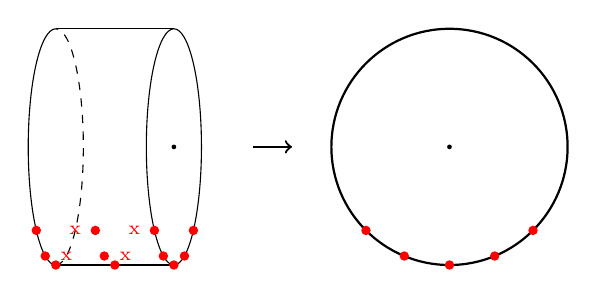
\begin{tikzpicture}
  			\draw (0, -2.0) -- (1.5, -2.0);% bottom line
  			\draw (0, 1) -- (1.5, 1);% top line
  			\draw[dashed] (0,-2.0) arc (-90:90:0.35 and 1.5); % left half of the left ellipse		
  			\draw (0, -2.0) arc (270:90:0.35 and 1.5);	% left half of the left ellipse		
  			\draw (1.5, -0.5) ellipse (0.35 and 1.5);	% right ellipse
  			
  			%	Center of right ellipse
  			\fill[black] (1.5, -0.5) circle (0.03cm);
  			
			\node[red] at (0.24748737341, 0.43933982822 - 2.0) {\scriptsize x};
			\node[red] at (0.13393920132, 0.11418070123 - 2.0) {\scriptsize x};
			
			\node[red] at (0.24748737341 + 0.75, 0.43933982822 - 2.0) {\scriptsize x};
			\node[red] at (0.13393920132 + 0.75, 0.11418070123 - 2.0) {\scriptsize x};
					
  			\foreach \x in {0.0, 0.75, 1.5} {
    			\foreach \angle in {-135, -90.0 - 22.5, -90.0, -45 - 22.5, -45} {
    			\pgfmathparse{\x<1.5 && \angle>-90.0}
        		%\typeout{\pgfmathresult}
    			\ifnum\pgfmathresult=0
    				\fill[red] ({0.35 * cos(\angle)}, {1.5 * sin(\angle)}) + (\x, -0.5) circle (0.06cm);
    			\else
    			\fi
    			}
			}
			
			\draw[->,thick] (2.5, -0.5) -- (3.0, -0.5);
			\draw[thick, color = black] (5.0, -0.5) circle [radius = 1.5];
			
			%	Center of right circle
			\fill[black] (5.0, -0.5) circle (0.03cm);
			
			\foreach \angle in {-135, -112.5, -90.0, -67.5, -45} {
				\fill[red] ({5.0 + cos(\angle) * 1.5}, {-0.5 + sin(\angle) * 1.5}) circle (0.06cm);
			}
		\end{tikzpicture}
	}
	\subfigure[Single hull point \textit{per} wheel (case 1)] {
		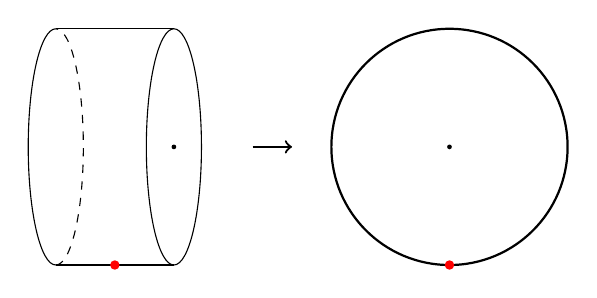
\begin{tikzpicture}
			\draw (0, -2.0) -- (1.5, -2.0);% bottom line
  			\draw (0, 1) -- (1.5, 1);% top line
  			\draw[dashed] (0,-2.0) arc (-90:90:0.35 and 1.5); % left half of the left ellipse		
  			\draw (0, -2.0) arc (270:90:0.35 and 1.5);	% left half of the left ellipse		
  			\draw (1.5, -0.5) ellipse (0.35 and 1.5);	% right ellipse
  			
  			%	Center of right ellipse
  			\fill[black] (1.5, -0.5) circle (0.03cm);
					
			%	Contact point of 3D wheel
    		\fill[red] (0.75, -2.0) circle (0.06cm);
			
			%	Arrow
			\draw[->,thick] (2.5, -0.5) -- (3.0, -0.5);
			
			%	Right circle			
			\draw[thick, color = black] (5.0, -0.5) circle [radius = 1.5];
			
			%	Center of right circle
			\fill[black] (5.0, -0.5) circle (0.03cm);
			
			%	Contact point
			\fill[red] (5.0, -2.0) circle (0.06cm);
		\end{tikzpicture}
	}
	\end{subfigmatrix}
	\caption{Hull points on each wheel}
    \label{fig:hullPoints}
\end{figure}

Apart from the restriction that every hull point must be above or at contact with the elevation map surface, the euler angle restrictions are linear and symmetrical. That means the lower and upper bound for each euler angle restriction is symmetrical (table \ref{tab:eulerAnglesRestrictions}).

\begin{wraptable}{r}{0.4\textwidth}
  \caption[Table caption shown in TOC.]{Euler angles restrictions.}
  \label{tab:eulerAnglesRestrictions}
  \renewcommand{\arraystretch}{0.8} % more space between rows
  \centering
  \begin{tabular}{ccc}
    \toprule
    $\roll_{max}$ [rad] & $\pitch_{max}$ [rad] & $\yaw_{max}$ [rad] \\
    \midrule
    $\frac{\pi}{4}$ & $\frac{\pi}{4}$ & $\pi$ \\
    \bottomrule
  \end{tabular}
\end{wraptable}

Below, the computed traversability maps are presented for case 1, under the conditions presented in this subsection. Traversability maps that match the results ranging from algorithm \ref{alg:slopeMinHeightMap} to \ref{alg:refinedMap} are presented, in order to enhance the differences among all maps. All the results presented below were obtained on an Intel® Core™ i7-10750H CPU @ 2.60GHz × 12 processor.

\begin{figure}[!ht]
    \centering
	\begin{subfigmatrix}{3}
	\subfigure[Algorithm \ref{alg:slopeMinHeightMap}, where $\yaw = 0$] {
    	\includegraphics[width=0.3\linewidth]{Figures/HeightMinPoints1.pdf}  
	}
	\subfigure[Algorithm \ref{alg:slopeMinHeightMapVarYaw}] {
    	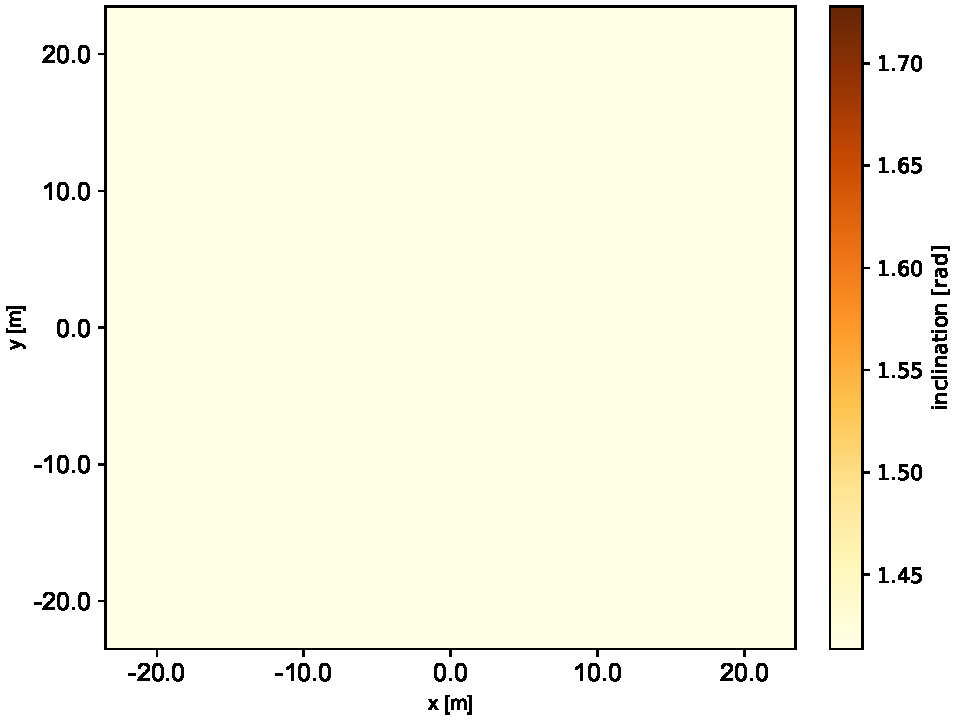
\includegraphics[width=0.3\linewidth]{Figures/HeightMin_maxInclinationPoints1.pdf}  
	}
	\subfigure[Algorithm \ref{alg:maxRoughnessMap}] {
    	\includegraphics[width=0.3\linewidth]{Figures/maxTerrainRoughness1.pdf}
	}
	\end{subfigmatrix}
    \caption{Traversability maps (case 1; map 1)}
    \label{fig:costMapsCase1Map1Alg2_4}
\end{figure}

\begin{figure}[!ht]
    \centering
	\begin{subfigmatrix}{2}
	\subfigure[Worst-case map] {
    	\includegraphics[width=0.48\linewidth]{Figures/worstCasePoints1.pdf}  
	}
	\subfigure[Algorithm \ref{alg:refinedMap}, where $r_s$ = 1 m and $C$ = 0.5] {
    	\includegraphics[width=0.48\linewidth]{Figures/mapRefinementPoints1.pdf}  
	}
	\end{subfigmatrix}
    \caption{Traversability maps (case 1; map 1)}
    \label{fig:costMapsCase1Map1Alg5}
\end{figure} 

The traversability maps which were obtained for case 2, are rendered in figure \ref{fig:costMapsCase2Alg2_4} and \ref{fig:costMapsCase2Alg5}. For the sake of brevity, these maps are presented in annex \ref{section:traversabilityMaps}, as they are graphically similar to the maps presented above \ref{section:traversabilityMaps}. The maximum terrain roughness map is the same both in case 1 and case 2.

\subsection{Discussion}
\label{subsection:costMapsDiscussion}

From the analysis of figures \ref{fig:costMapsCase1Map1Alg2_4} and \ref{fig:costMapsCase1Map1Alg5}, it is noticeable an improvement of the traversability classification of the terrain, as it expected that locations with high vertical gradient feature a high traversability cost. Tables  presents the correlation between $\nabla \FunctionElevation(\cdot)$ and $\FunctionTraversability(\cdot)$ for each map of figures \ref{fig:costMapsCase1Map1Alg2_4} and \ref{fig:costMapsCase1Map1Alg5}.

\begin{table}[!htb]
  \caption{Comparison between algorithms \ref{alg:slopeMinHeightMap} and \ref{alg:slopeMinHeightMapVarYaw} (case 1).}
  \label{tab:ResultsAlg2_and_3_case1}
  \centering
  \renewcommand{\arraystretch}{1.2} % more space between rows
  \begin{tabular}{@{}rrrcrr@{}} % remove space to the vertical edges @{}...@{}
    \toprule
      & \multicolumn{2}{c}{Map 1} & \phantom{abc} & \multicolumn{2}{c}{Map 2} \\
    \cmidrule{2-3}
    \cmidrule{5-6}
    $\text{Algorithm}$ & $\text{2}$ & $\text{3}$ && $\text{2}$ & $\text{3}$ \\
    \midrule
      $\text{[ms] / cell}$ & 3.10 $\pm$ 4.61 & 0.16 && 0.36 & 0.71 \\
      $\text{iterations / cell}$ & 9.12 $\pm$ 11.55 & 0.16 && 0.36 & 0.71 \\
      $\text{optimality}$ & 0.01 $\pm$ 0.05 & 50.04 && -9.07 & 29.09 \\
      $\nabla \FunctionElevation(\cdot) \text{ vs }\FunctionTraversability(\cdot) \text{ [R]}$ & 0.89 & -50.96 && 12.22 & -63.54 \\
    \bottomrule
  \end{tabular}
\end{table}

\begin{table}[!htb]
  \caption{Comparison between algorithms \ref{alg:slopeMinHeightMap} and \ref{alg:slopeMinHeightMapVarYaw} (case 2).}
  \label{tab:ResultsAlg2_and_3_case2}
  \centering
  \renewcommand{\arraystretch}{1.2} % more space between rows
  \begin{tabular}{@{}rrrcrr@{}} % remove space to the vertical edges @{}...@{}
    \toprule
      & \multicolumn{2}{c}{Map 1} & \phantom{abc} & \multicolumn{2}{c}{Map 2} \\
    \cmidrule{2-3}
    \cmidrule{5-6}
    $\text{Algorithm}$ & $\text{2}$ & $\text{3}$ && $\text{2}$ & $\text{3}$ \\
    \midrule
      $\text{[ms] / cell}$ & 0.07 & 0.16 &&  0.36 & 0.71 \\
      $\text{iterations / cell}$ & 9.12 $\pm$ 11.55 & 0.16 && 0.36 & 0.71 \\
      $\text{optimality}$ & -0.86 & 50.04 && -9.07 & 29.09 \\
      $\nabla \FunctionElevation(\cdot) \text{ vs }\FunctionTraversability(\cdot) \text{ [R]}$ & 14.27 & -50.96 && 12.22 & -63.54 \\
    \bottomrule
  \end{tabular}
\end{table}

\begin{table}[!htb]
  \caption{Comparison between algorithms \ref{alg:maxRoughnessMap} and \ref{alg:refinedMap} (case 1).}
  \label{tab:ResultsAlg4_and_5_case1}
  \centering
  \renewcommand{\arraystretch}{1.2} % more space between rows
  \begin{tabular}{@{}rrrcrr@{}} % remove space to the vertical edges @{}...@{}
    \toprule
      & \multicolumn{2}{c}{Map 1} & \phantom{abc} & \multicolumn{2}{c}{Map 2} \\
    \cmidrule{2-3}
    \cmidrule{5-6}
    $\text{Algorithm}$ & $\text{4}$ & $\text{5}$ && $\text{4}$ & $\text{5}$ \\
    \midrule
    $\text{[ms] / cell}$ & 0.07 & 0.16 &&  0.36 & 0.71 \\
    $\nabla \FunctionElevation(\cdot) \text{ vs }\FunctionTraversability(\cdot) \text{ [R]}$ & 14.27 & -50.96 && 12.22 & -63.54 \\
    \bottomrule
  \end{tabular}
\end{table}

\begin{table}[!htb]
  \caption{Comparison between algorithms \ref{alg:maxRoughnessMap} and \ref{alg:refinedMap} (case 2).}
  \label{tab:ResultsAlg4_and_5_case2}
  \centering
  \renewcommand{\arraystretch}{1.2} % more space between rows
  \begin{tabular}{@{}rrrcrr@{}} % remove space to the vertical edges @{}...@{}
    \toprule
      & \multicolumn{2}{c}{Map 1} & \phantom{abc} & \multicolumn{2}{c}{Map 2} \\
    \cmidrule{2-3}
    \cmidrule{5-6}
    $\text{Algorithm}$ & $\text{4}$ & $\text{5}$ && $\text{4}$ & $\text{5}$ \\
    \midrule
    $\text{[ms] / cell}$ & 0.07 & 0.16 &&  0.36 & 0.71 \\
    $\nabla \FunctionElevation(\cdot) \text{ vs }\FunctionTraversability(\cdot) \text{ [R]}$ & 14.27 & -50.96 && 12.22 & -63.54 \\
    \bottomrule
  \end{tabular}
\end{table}

As it is expected, the computational burden increases a lot, when the algorithms are run for case 2, because the \acrshort{nlp} needs to account for more constraints.

\section{Path planning}
\label{section:pathPlanning}

Up to now, it is possible to compute a potential flow with respect to the cost maps presented in subsection \ref{subsection:costMapImplementation}. These cost maps replace function $\speedFunction\cdot$  in the Eikonal equation from \ref{eq:eikonalEquation}, which outputs a gradient function, $\nabla \timeFunction\cdot$, that enables the computation of an optimal path towards the selected goal.

Each value that is assigned to every cell on the cost map expresses the fact that it is safer or riskier to pass by that position. If $\speedFunction\cdot$ presents a high (low) value to some cell of the cost map, that means if is safer (riskier) to cross that position. Therefore, $\nabla \timeFunction\cdot$ will be lower (higher) for that same position, because it will take more time to reach some goal point from the selected position, as it is more dangerous (and slower) to go through it. In future sections of this thesis, this information will help a mobile robot to carefully assess, plan and adapt its motion according to the features of the terrain it is at, and plans to go through.

\subsection{Implementation}
\label{subsection:implementationfm}

After the discretization of gradient $\nabla u$, the optimal path comes as,

\begin{equation}
	\alpha = \arctan \frac{\frac{\partial}{\partial y} u(p_i)}{\frac{\partial}{\partial x} u(p_i)}
\end{equation}

\begin{equation}
	p_{i+1, \; x} = p_{i, \;x} - cos(\alpha)
\end{equation}

\begin{equation}
	p_{i+1, \; y} = p_{i, \;y} - sin(\alpha)
\end{equation}